\documentclass[conference]{IEEEtran}
\IEEEoverridecommandlockouts
% The preceding line is only needed to identify funding in the first footnote. If that is unneeded, please comment it out.
\usepackage{cite}
\usepackage{amsmath,amssymb,amsfonts}
\usepackage{algorithmic}
\usepackage{graphicx}
\usepackage{textcomp}
\usepackage{xcolor}
\def\BibTeX{{\rm B\kern-.05em{\sc i\kern-.025em b}\kern-.08em
    T\kern-.1667em\lower.7ex\hbox{E}\kern-.125emX}}
\begin{document}

\title{Forecasting Total Energy Consumption in the Swiss Energy Grid}

\author{
\IEEEauthorblockN{Matthias Minder}
\IEEEauthorblockA{matthias.minder@epfl.ch}
\and
\IEEEauthorblockN{Yves Rychener}
\IEEEauthorblockA{
yves.rychener@epfl.ch}}


\maketitle

\begin{abstract}
TODO
\end{abstract}


\section{Introduction}
The energy grid is a highly complex network that has to be tightly controlled by the so-called grid operator in order to assure its well-functioning. In particular, energy consumption has to be at equilibrium with production at all times to avoid blackouts with possibly fatal consequences. It is therefore of great interest to accurately model and forecast the energy consumption, such that the energy made available to the grid can be adjusted accordingly. Moreover, long-term forecasting is of interest to adjust the energy strategy: How much power plants will be needed in the future and should be built? 
\par
Within the scope of this work, we therefore aim to generate accurate forecasts for the total energy consumption of the Swiss energy grid. To this effect, we analyze the quarter-hourly grid data between 2009 and 2019 available from the Swiss grid operator, Swissgrid [CITATION!!!]. We start with weekly integrated data before we move on to daily integrated data before tackling the quarter-hourly energy consumption data, thus increasing the model complexity step by step. We thereby hope to create more and more accurate models for the data that are able to capture both long- and short term trends in order to finally create accurate forecasts. REWRITE!!!
\par
In order to compare forecast accuracy between the models, we construct our models on the data up to and including 2017. We then assess the accuracy of the forecasts on the data of the year 2018 for model comparison. 
\par


%Furthermore, we rely on the Akaike information criterion (AIC) for estimation of the quality of a given model. 
%The work will be structured as follows: In the second chapter, we present exploratory analysis of the data to identify sensible models. In the third chapter, we then [ DO WHAT?!?]. 

\section{Data Exploration}
\begin{figure*}[ht]
	\centering
	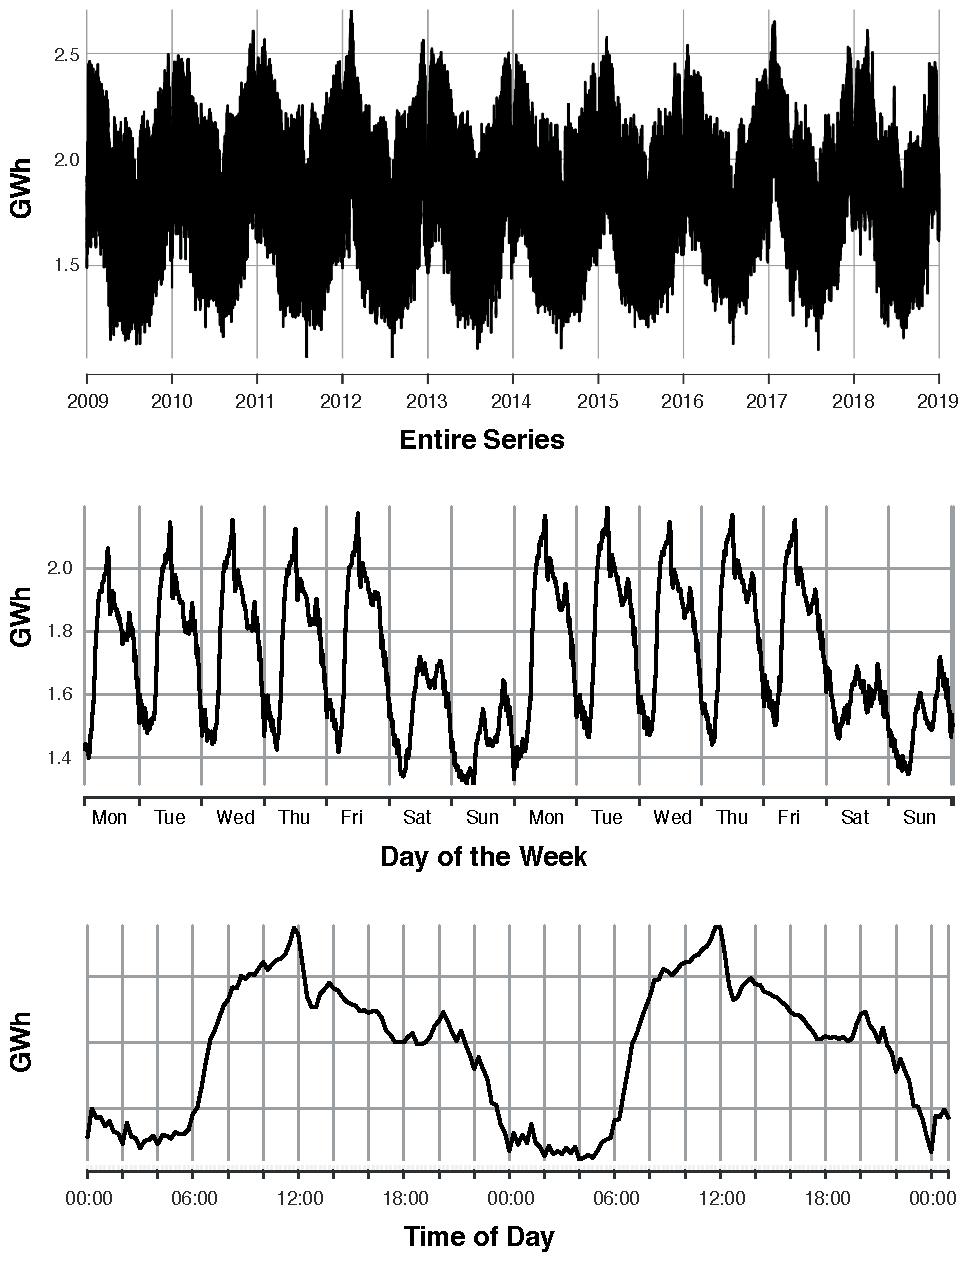
\includegraphics[width=0.8\textwidth]{Figs/Fig1.pdf}
	\caption{Total consumption in the Swiss Energy Grid, showing the entire series, two example weeks and two example work days.}
	\label{SeriesPlot}
\end{figure*}
We start off our analysis with an exploratory data analysis. The full time series for energy consumption together with representative weeks and days are shown in \ref{SeriesPlot}. From the plots, it becomes apparent that there are multiple levels of seasonality present in the data. First of all, we see a roughly sinusoidal yearly variation, with higher values during winter months than summer. Secondly, we see a weekly repetitive pattern, with lower energy consumption during the week-end as compared to the work days. Finally, we see a highly irregular daily pattern with the highest energy consumption right before lunchtime.
\par
Moreover, on the plot of the full time series we observe a sharp drop in energy consumption around Christmas and New Year. The same applies for other public holidays such as the first of August or  easter. Note that the public holidays vary from canton to canton, but the following ones are common to most cantons: January first and second, Good Friday, Easter Monday, Ascension, Pentecost Monday, the first of August (the Swiss national day), and finally the 25. and 26 of December. 
\par

\par


\section{Weekly Integrated Data}
We begin by considering weekly integrated data. A plot of the resulting time series can be seen in Figure \ref{weekly}. The integrated data only exhibits a yearly seasonality, whereas the daily and weekly seasonal patterns are removed through the integration. There are multiple approaches that can be considered in order to allow for that seasonality, three of which are outlined in the following sections. Moreover, from the plot in Figure \ref{weekly} it becomes apparent that the energy consumption systematically drops in the weeks around New Year. In order to take this into account, we label weeks that end between December 25th and January 8th as holiday weeks and treat them specially. 

\begin{figure*}[ht]
	\centering
	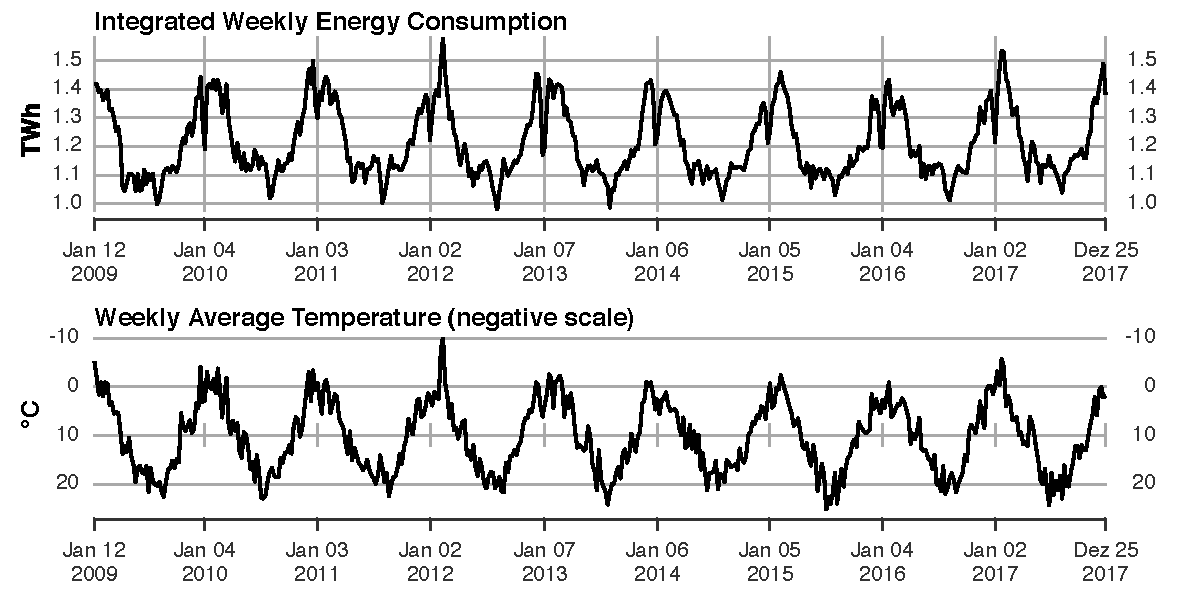
\includegraphics[width=1\textwidth]{Figs/weeklyInt+Temperature.pdf}
	\caption{}
	\label{weekly}
\end{figure*}

\subsection{Modeling Seasonality with Sine and Cosine}
A simple, intuitive approach is to regress out a sinusoidal pattern while fitting an ARIMA($p$, $d$, $q$) model to the data. This was done by regressing against sine and cosine terms with periodicity $T=365.25 / 7 \simeq 52$, corresponding to a yearly oscillation with unknown phase. Moreover, to capture harmonics, $T / 2$ up to $T / 5$ were also added to the fit. Finally, an indicator variable for the holiday season was added to capture the special behavior during that period. This first model will be referred to as model W1.
\par
The ACF and PACF of the regression residuals can be seen on the left side of Figure \ref{weekly_mod1}. The ACF of the residuals still shows some periodic structure, which is not completely removed through differencing. This seasonal structure is not present in the PACF. Looking at the ACF and PACF plots, it is not obvious what the optimal ARIMA parameters are, but $p=6$, $d=1$ and $q=4$ seem to be a reasonable choice. 
\par
Fitting an ARIMA(6,1,4) model with the aforementioned regressors yields an AIC of 2586.7. The model diagnostics can be seen on the right side of Figure \ref{weekly_mod1}. A visual inspection of the standardized residuals and ACF suggests that no apparent seasonal patterns remain after model fitting. Moreover, the p-values of the Ljung-Box indicate that the residuals do not exhibit serial correlation. The cumulative periodogram suggests that the residuals are white noise. However, the Q-Q plot of the residuals exhibits heavy tails, suggesting that the residuals do not follow a normal distribution.
\begin{figure*}[ht]
	\centering
	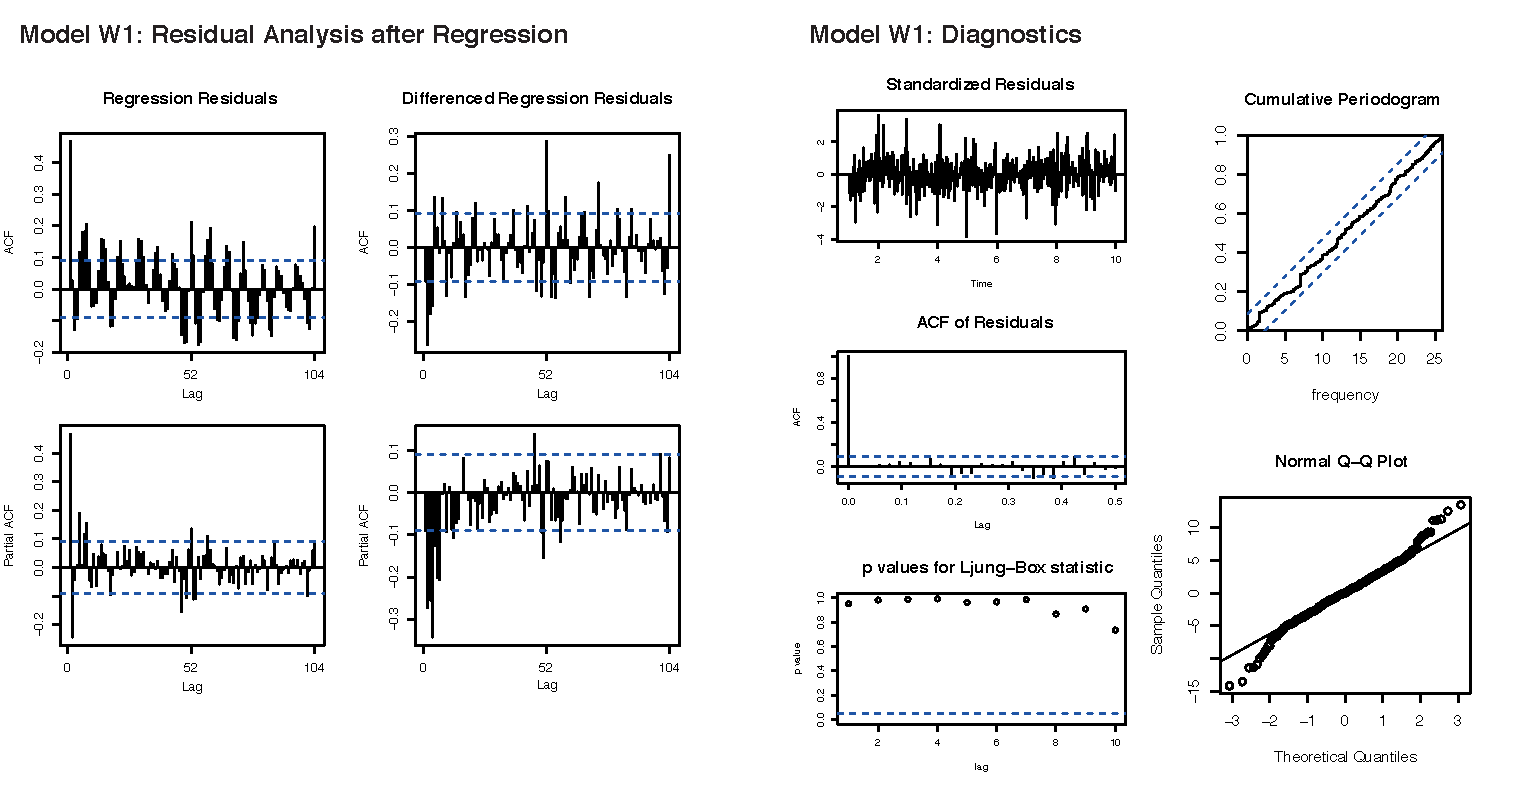
\includegraphics[width=1\textwidth]{Figs/Fig3.pdf}
	\caption{}
	\label{weekly_mod1}
\end{figure*}

\subsection{Modeling Seasonality with Temperature}
Considering Figure \ref{weekly}, we can see that the weekly energy consumption follows closely the negative average temperature. We therefore use the weekly average temperature in addition to the holiday indicator as a regressor when fitting a second ARIMA model. This model will be referred to as model W2.
\par
Figure \ref{weekly_mod2} shows on the left side the ACF and the PACF of the residuals after the regression. The ACF of the residuals indicates that there is some residual periodicity, manifested by oscillations with period 52 (corresponding to one year) in the plot. The PACF however seems well-behaved. These plots suggest an ARMA(1,4) model, where the results have to be treated with care due to the residual oscillations. Differencing lead to a slightly better behaved ACF, although the periodicity remains. However the PACF that was before well-behaved now seems probematic, with many significant values at a large lag. These plots suggest an ARIMA(4, 1, 1) model.
\par
We fit both the ARMA(1,4) and the ARIMA(4,1,1) model and compare them in terms of AIC. With an AIC of 2555.8, the model without differencing outperforms the integrated model with an AIC of 2562.5. The diagnostic plots for the ARMA model can be found on the right side of Figure \ref{weekly_mod2} and do not suggest any problems with the model. In particular, compared to the model W1, the residual distribution seems to be more close to a normal. Also note that the AIC increased by around 30. 

\begin{figure*}[ht]
	\centering
	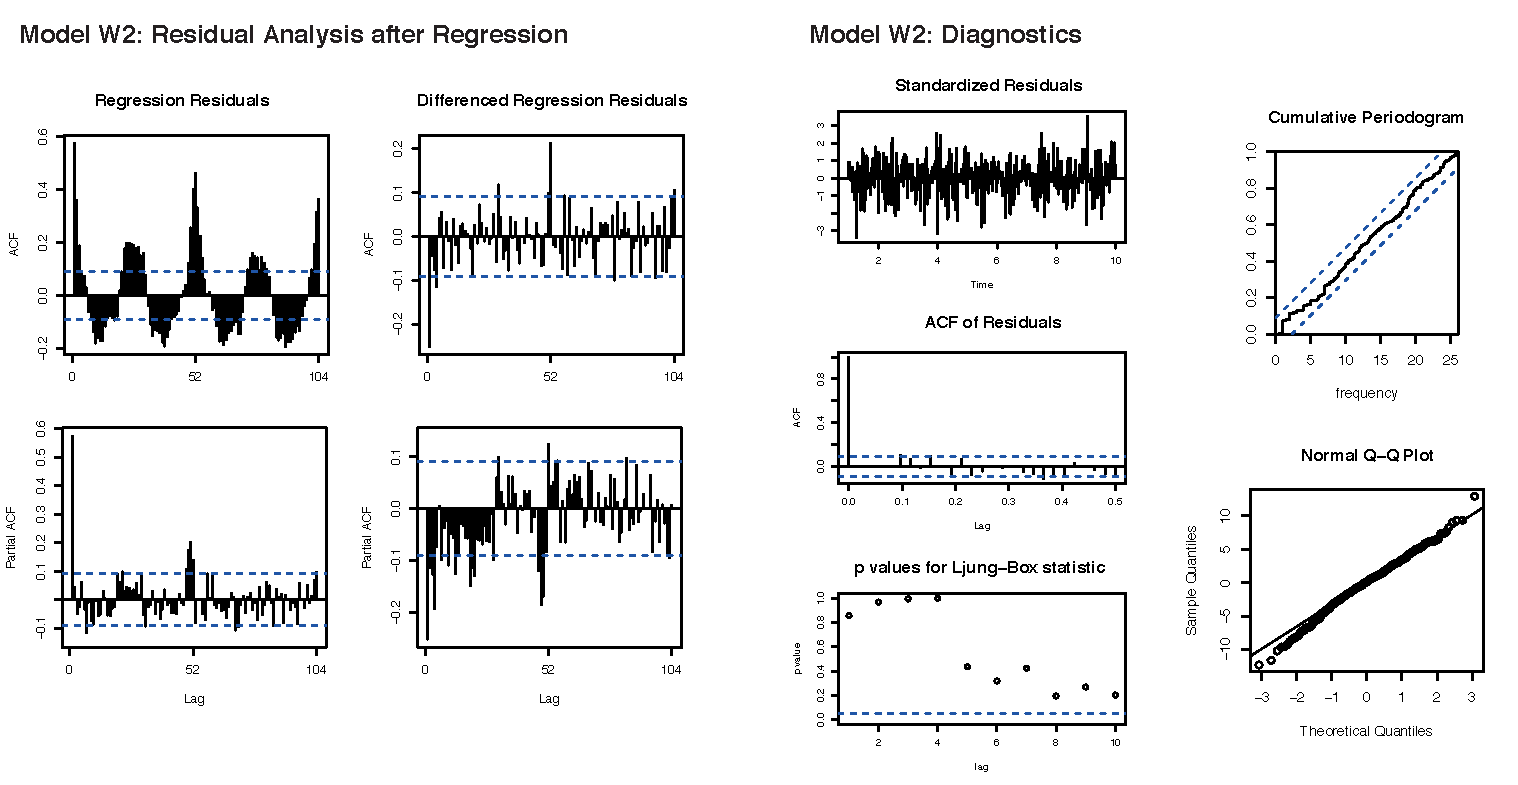
\includegraphics[width=1\textwidth]{Figs/Fig4.pdf}
	\caption{}
	\label{weekly_mod2}
\end{figure*}

\subsection{Modeling Seasonality with SARIMA}
We can also model the seasonality using a seasonal ARIMA model with a 52 week seasonality. The ACF and PACF plots suggest taking D=1. After seasonal differencing, the ACF and PACF suggest taking a SMA(2) model. The non-sesonal component is less clear and we settle on an ARMA(1,2) model. The resulting model is SARIMA(1,0,2)(0,1,2)\textsubscript{52}. The resulting diagnostic plots look good with slight non-guassianity in the qq-plot. The AIC is 2312.1, which is substantially better than the other models examined before.

\section{15min Data}
We now look at the data in the 15 minute timeframe. This is the timeframe provided by SWISSGRID. When we look at the time series itself and the ACF plot in figure \ref{15min}, we can see that there are at least 3 seasonalities. They are daily (lag 96), weekly (lag 672) and yearly (lag 35040). This also aligns with our intuition: In addition to the weekly patterns (weekend) and yearly patterns (summer-winter), we expect to have a daily pattern (day-night).
\subsection{Modeling Seasonality with TBATS}
Normal SARIMA models don’t support multiple seasonalities. We therefore resort to another model called TBATS (\textbf{T}rigonometric, \textbf{B}ox-Cox transform, \textbf{A}RMA errors, \textbf{T}rend and \textbf{S}easonal components) proposed by De Livera, Alysha M., Rob J. Hyndman and Ralph D. Snyder \cite{TBATS_paper}. The TBATS model uses a Fourier series to model each seasonality. Box-Cox transformations are also incorporated and the residuals are modeled using an ARMA model.
The result is not convincing however. The residuals are clearly neither gaussian nor white noise (Figure \ref{15min}). Clearly, more work would have to be done to obtain a good result here. For example, one could use the predictions from our previous models for higher time-frames as covariates for a model. After obtaining the prediction for the day, we could limit ourself to just modeling the daily evolution. However we would have to take into account the fact that weekends have a different pattern than weekdays. Also, the confidence bands  of the `forecast`-function could not be trusted at all, since they don’t take into account uncertainty of the exogenous variable.

\begin{thebibliography}{00}

\bibitem{TBATS_paper}
De Livera, Alysha M., Rob J. Hyndman, and Ralph D. Snyder. "Forecasting time series with complex seasonal patterns using exponential smoothing." Journal of the American Statistical Association 106.496 (2011): 1513-1527.
APA	

\end{thebibliography}

\end{document}


% TODO: 
% Citations
% Short explanation of ARIMA, SARIMA, parameters
% Describe where temperature data comes from.
% Remove all traces of 15min-data